\section{Live-system evaluation on held-out emails}
\label{ch:live}

This chapter measures the deployed agent itself (Section~\ref{sec:post-evaluation-changes}) on real student emails. The controlled experiment of the preceding chapters tests one retrieval decision on a fixed retrieve-then-generate configuration. The live evaluation was done step by step over eleven numbered development stages (Stage 1 to Stage 11, successive versions of the system), and its protocol was not fixed in advance (not pre-registered). Its numbers must not be combined with those of the controlled study. The data are private, so only aggregate counts are reported.

\subsection{Purpose and difference from the controlled protocol}

The question is how well the deployed agent answers real student emails, and whether the result holds beyond the emails on which the system was developed. The evaluation differs from the controlled protocol in four ways.

\begin{itemize}
  \item \textbf{Full agent.} Each question is sent to the production chat API on a test copy of the production system. The agent decides when to call the knowledge-base search tool (FAQs and document passages, reranked against the original question) and which structured tools to use (announcements, curricula, syllabi, rooms, staff, schedules). It runs under the production prompts. The model is GPT-6 Luna, a newer version of the GPT-5.6 Luna model used in the controlled experiment, with reasoning disabled.
  \item \textbf{Latest message only.} Every request is a new conversation with one user message. Follow-up turns are tested separately (Section~\ref{sec:live-memory}).
  \item \textbf{Tool evidence.} From the stage labelled ``first run with tool evidence'' (Stage~9 in Figure~\ref{fig:live-stages}), judges see each tool's output as well as the answer.
  \item \textbf{No pre-registration.} Thresholds, prompts and knowledge-base content changed between runs, and the reference is a snapshot of a growing knowledge base. The live configuration cannot be replayed, and no fixed copy of it exists.
\end{itemize}

\subsection{Question sets}

All email questions come from the anonymized archive of 1,693 email and reply pairs described in Chapter~\ref{ch:data} (see Figure~\ref{fig:eval-dataflow}). Four email sets and two monitoring sets were used (Table~\ref{tab:live-sets}). A set is clean if no fix had been aimed at it before it was measured. It is contaminated once fixes were made for failures seen on it.

\begin{table}[htbp]
\centering
\caption[Question sets of the live evaluation]{Question sets of the live evaluation. Email sets have no overlap.}
\label{tab:live-sets}
\small
\begin{tabularx}{\linewidth}{@{}>{\raggedright\arraybackslash}p{0.17\linewidth}r>{\raggedright\arraybackslash}X@{}}
\toprule
Set & $N$ & Origin and status \\
\midrule
Tuned emails & 334 & 158 emails from the hand-picked 240-email review pool (Chapter~\ref{ch:data}), after leaving out personal-record requests, spam and duplicates, and 176 from a second selection of about nine emails per topic group outside that pool. Reviewed during development, and every early fix and confirmed fact came from them, so the set is contaminated. \\
Holdout 1 & 271 & Drawn at random by topic group from the remaining emails (Appendix~\ref{app:live-sampling}). Measured before any fix was aimed at it, but later fixes used its failures. Contaminated after its first measurement. \\
Holdout 2 & 275 & Drawn after holdout 1 in the same way, and asked twice before fixes. Contaminated after the fixes aimed at it. \\
Holdout 3 & 298 & The last unused archive emails. No fix was tuned on them. Final clean set. \\
Real traffic & 109 & First question of each real conversation in a 30-day window before the first monitoring measurement. Used to find faults, so not held out. \\
Recent chats & 38 & New first questions arriving after the real-traffic window. Partly used for fixes. \\
\bottomrule
\end{tabularx}
\end{table}

The held-out sets were drawn with a fixed seed, and spread over 24 topic groups of the archive so that every topic is covered. The archive was already anonymized, and an extra pass by two language-model agents removed any names and signatures that were left (Appendix~\ref{app:live-sampling}). Rows that were not student questions were dropped, so the third set has 298 of the 303 eligible emails.

\subsection{Grading}

AI agents graded the answers blind, with labels shuffled per row and up to three runs graded side by side. The rows were split into chunks of about 33, and one judge agent graded each chunk. Every answer therefore received one grade, and no vote was taken. Holdout 3 used nine agents, the Sonnet regrades of holdouts 1 and 2 used six and eight, and the decision-model test used four. The decision model is a model that answers yes or no for each passage, and its probability is the ranking score (Section~\ref{sec:live-decisions}). The original gradings of holdouts 1 and 2 and of the tuned-set runs used Claude Opus 5.5 judges (Opus from here on). The final set and the hedge experiment (a test of a prompt rule against vague answers, Section~\ref{sec:live-ab}) used Claude Sonnet 5.5 judges (Sonnet). Holdouts 1 and 2 were later regraded with Sonnet judges under the current rubric on the same blinded inputs, so all five clean runs share one judge model and one rubric. No human grades were collected.

\textbf{Truth sources.} Judges compare each answer with the current FAQ snapshot (104 FAQs from Stage~10, grown from 74), the link table (the list of official links), syllabi, the scope policy (the rules on which questions the bot should answer), facts confirmed by the author and the staff reply. The staff reply is only a hint and may be out of date. A fact counts as available only if one of these sources states it.

\textbf{Grades.} Each answer receives exactly one of five grades. Table~\ref{tab:live-grades} defines them and shows how each one enters the reported rates. The grades differ from the categories of the controlled experiment (Chapter~\ref{ch:methodology}), and the two sets of results are never combined.

\begin{table}[htbp]
\centering
\caption[The five grades of the live evaluation and how they are counted]{The five grades of the live evaluation and how they are counted. Graded rows are all rows except \textsc{N/A}. The correct rate is \textsc{Correct} divided by the graded rows, and the wrong rate is \textsc{Wrong} divided by the graded rows.}
\label{tab:live-grades}
\small
\begin{tabularx}{\linewidth}{@{}>{\raggedright\arraybackslash}p{0.13\linewidth}>{\raggedright\arraybackslash}X>{\raggedright\arraybackslash}p{0.27\linewidth}@{}}
\toprule
Grade & Meaning & How it is counted \\
\midrule
\textsc{Correct} & The answer gives the main available fact or procedure and contradicts nothing. & Good. Counts toward the correct rate. \\
\textsc{Partial} & The answer gets some main fact right, but an important part is missing or buried in hedging (vague wording that avoids stating a rule plainly). & Partly good. Counts against the correct rate but not toward the wrong rate. \\
\textsc{Wrong} & The answer gives none of an available main fact, contradicts one, states an outdated rule, or adds a specific detail (amount, date, URL, procedure) that no source supports. & Bad. Counts toward the wrong rate. \\
\textsc{Gap} & No source states the needed fact, and the answer handles this reasonably, for example by referring the student to the right office without inventing facts. & A loss caused by missing knowledge, not by the answer. Counts against the correct rate but not toward the wrong rate. \\
\textsc{N/A} & The email is not a real question for the bot (thanks, spam), or it asks about a personal record that only staff can see and the answer correctly refers the student. & Left out of all rates. \\
\bottomrule
\end{tabularx}
\end{table}

Two rules separate neighboring grades. An answer that gives part of an available fact is \textsc{Partial}, and one that gives none of it is \textsc{Wrong}. When no source covers the question, a reasonable answer is \textsc{Gap}, but an answer that invents a specific detail is \textsc{Wrong}. Judges also set two flags, which do not change the grade. The hedge flag marks an answer that avoids or defers a fact that was available. The noise flag marks an answer that adds unneeded or off-topic detail. The flags are used only to explain \textsc{Partial} answers (Section~\ref{sec:live-failures}). The original Opus grading of holdout 1 used an older rubric that counted a correct personal-record referral as \textsc{Gap}. The current rubric counts it as \textsc{N/A}.

For agreement between judges, the grades are compared in two ways: all five grades, and correct versus not correct, where \textsc{Partial}, \textsc{Wrong} and \textsc{Gap} are all not correct.

\textbf{Evidence and reliability.} Before Stage~9, judges saw no tool output, which turned most tool-based answers into \textsc{Gap}. From Stage~9 on they see each answer's tool output (at most 4,000 characters per output and 12,000 per answer). Two independent sets of judges on the same 109 traffic answers agreed exactly on 98 rows (89.9 percent, Cohen's $\kappa=0.76$) and on 102 rows for correct versus not correct. Judges were unreliable at judging whether a detail was invented. At Stage~10, nine of 22 email rows called wrong for an invented date or URL were supported by the answer's own tool output. A script therefore checks every date, amount, URL and email address against the question and the full tool output (Appendix~\ref{app:live-check}). After one data fix for a guessed announcement URL, it flagged seven and six rows on the two runs of holdout 3 (plus four and three with only relative dates). All of them were derived details and none was invented. It also found a real defect. The bot sometimes rewrote long announcement URLs and broke them (Section~\ref{sec:live-ab}). The second measurement of holdout 2 and the hedge experiment were not checked this way.

\textbf{Run-to-run variation.} The same configuration run twice (runs $a$ and $b$) on holdout 2 differs in grade on 32 of 275 rows (12 percent, Opus grading), mostly between \textsc{Correct} and \textsc{Partial}. Between the two runs of a set, the correct rate differs by 0.3 to 1.9 points (Table~\ref{tab:live-holdout} and Appendix~\ref{app:live-grader}). Differences below about three points between single runs are treated as noise.

\subsection{Results on clean held-out sets}

\begin{table}[htbp]
\centering
\caption[Grades on the held-out email sets]{Grades on the held-out email sets. Counts are \textsc{Correct}, \textsc{Partial}, \textsc{Wrong}, \textsc{Gap} and \textsc{N/A}, and percentages are of graded rows. Runs $a$ and $b$ are two repeated runs of the same configuration. The five clean held-out rows were graded by Sonnet under the current rubric. The tuned row and the rows marked $\dagger$ were graded by Opus. Rows marked $\dagger$ were measured after fixes aimed at the set and are not clean.}
\label{tab:live-holdout}
\small
\setlength{\tabcolsep}{4pt}
\begin{tabular}{@{}llrrrrrrrr@{}}
\toprule
Set & Run & $N$ & C & P & W & \textsc{Gap} & N/A & Correct \% & Wrong \% \\
\midrule
Tuned emails (Stage 11, Opus) & 1 & 334 & \multicolumn{5}{c}{not counted} & 87.8 & 1.3 \\
Holdout 1 & 1 & 271 & 165 & 35 & 4 & 30 & 37 & 70.5 & 1.7 \\
Holdout 2 & $a$ & 275 & 191 & 19 & 4 & 34 & 27 & 77.0 & 1.6 \\
Holdout 2 & $b$ & 275 & 191 & 19 & 2 & 35 & 28 & 77.3 & 0.8 \\
Holdout 3 & $a$ & 298 & 205 & 22 & 3 & 38 & 30 & 76.5 & 1.1 \\
Holdout 3 & $b$ & 298 & 206 & 19 & 8 & 38 & 27 & 76.0 & 3.0 \\
\midrule
Holdout 2$^\dagger$ (Opus) & $a$ & 275 & \multicolumn{5}{c}{not counted} & 84.6 & 3.2 \\
Holdout 2$^\dagger$ (Opus) & $b$ & 275 & \multicolumn{5}{c}{not counted} & 83.0 & 3.2 \\
\bottomrule
\end{tabular}
\end{table}

% Correct rates with Wilson 95% intervals for the tuned set and the five clean held-out runs.
% x = (percent - 60) * 0.3 cm, so the axis spans 60 to 95 percent over 10.5 cm.
\begin{figure}[htbp]
\centering
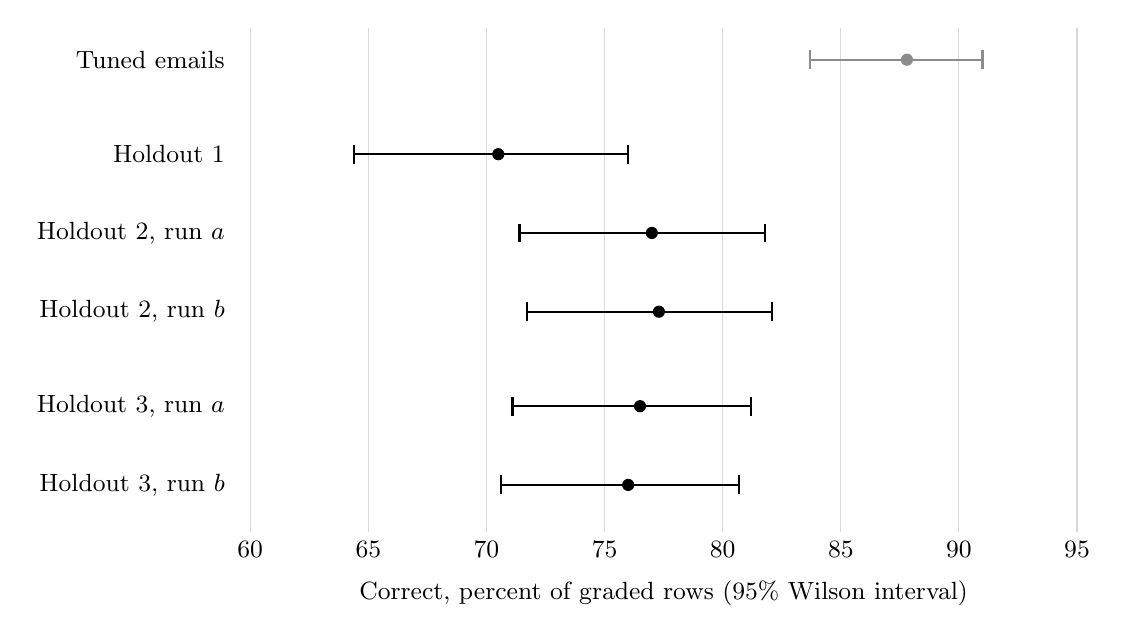
\begin{tikzpicture}[x=1cm,y=1cm,font=\small]
  \foreach \p in {60,65,70,75,80,85,90,95} {
    \draw[black!15] ({(\p-60)*0.3},0.4) -- ({(\p-60)*0.3},-6.0);
    \node[below] at ({(\p-60)*0.3},-6.0) {\p};
  }
  \node[below] at (5.25,-6.5) {Correct, percent of graded rows (95\% Wilson interval)};
  \foreach \y/\lab/\lo/\pt/\hi/\sty in {
      0/Tuned emails/83.7/87.8/91.0/black!45,
     -1.2/Holdout 1/64.4/70.5/76.0/black,
     -2.2/{Holdout 2, run $a$}/71.4/77.0/81.8/black,
     -3.2/{Holdout 2, run $b$}/71.7/77.3/82.1/black,
     -4.4/{Holdout 3, run $a$}/71.1/76.5/81.2/black,
     -5.4/{Holdout 3, run $b$}/70.6/76.0/80.7/black} {
    \node[left,align=right] at (-0.2,\y) {\lab};
    \draw[\sty,line width=.8pt] ({(\lo-60)*0.3},\y) -- ({(\hi-60)*0.3},\y);
    \draw[\sty,line width=.8pt] ({(\lo-60)*0.3},\y-0.12) -- ({(\lo-60)*0.3},\y+0.12);
    \draw[\sty,line width=.8pt] ({(\hi-60)*0.3},\y-0.12) -- ({(\hi-60)*0.3},\y+0.12);
    \fill[\sty] ({(\pt-60)*0.3},\y) circle (2.2pt);
  }
\end{tikzpicture}
\caption[Correct rates of the deployed agent on the tuned emails and on the five clean held-out runs, with Wilson 95 percent intervals]{Correct rates of the deployed agent on the tuned emails and on the five clean held-out runs, with Wilson 95 percent intervals (a confidence interval for a percentage). The five clean runs were graded by Sonnet under the current rubric. The tuned emails (grey) were graded by Opus, supplied the fixes and are contaminated. The intervals of all clean runs overlap, while the tuned set lies higher.}
\label{fig:live-holdout}
\end{figure}


Table~\ref{tab:live-holdout} and Figure~\ref{fig:live-holdout} give the central result. On sets the fixes had not targeted, the deployed agent was graded correct on 70.5 to 77.3 percent of graded questions (roughly three quarters) and wrong on 0.8 to 3.0 percent. Four runs lie within 1.3 points of each other. Holdout 1 is lower, but it was measured at an earlier development stage, so its rate may reflect the system as well as the sample. Each run has sampling uncertainty of about five points. For example, the Wilson 95 percent interval (a standard confidence interval for a percentage) is 64.4 to 76.0 percent for holdout 1 and 71.7 to 82.1 percent for holdout 2 run $b$. All five clean intervals overlap.

The tuned set was measured at Stage~11 alongside the first holdout with Opus judges. It scored 87.8 percent correct (95 percent interval 83.7 to 91.0) and 1.3 percent wrong, against 76.3 and 2.3 percent on the first holdout under the same Opus grading. The tuned set therefore overstates how well the system does on new emails by 11.5 points. Most of the difference is in \textsc{Gap}. \textsc{Gap} was 7 percent of graded rows on the tuned set (21 of 312) and 13 percent on the first holdout.

The judge model changes the correct rate by a few points. The Opus gradings of the same answers were higher than the Sonnet gradings by 1.6 to 5.8 points, and the two agreed exactly on 81.6 percent of holdout 2 answers (Appendix~\ref{app:live-grader}). The clean runs are therefore compared only with each other.

The fixes aimed at the second holdout's failures raised it to 84.6 and 83.0 percent. Those runs were graded against the updated knowledge-base snapshot. The answers from before the fixes, graded in the same blind batch against the same snapshot, scored 72.7 percent correct and 10.7 percent wrong. The 11-point gain therefore comes partly from the fixes and partly from the changed reference, and it is not an estimate for new emails. The final set, untouched by any fix, returned 76.5 and 76.0 percent. This compares different sets and judges and does not measure transfer. Between 27 and 37 rows per clean run are N/A.

\subsection{Tuned sets and development history}

% Correct and wrong percent by development stage on the 334 tuned emails (values of Table tab:live-history).
% x = (stage - 1) * 0.9 cm, y = percent * 0.055 cm.
\begin{figure}[htbp]
\centering
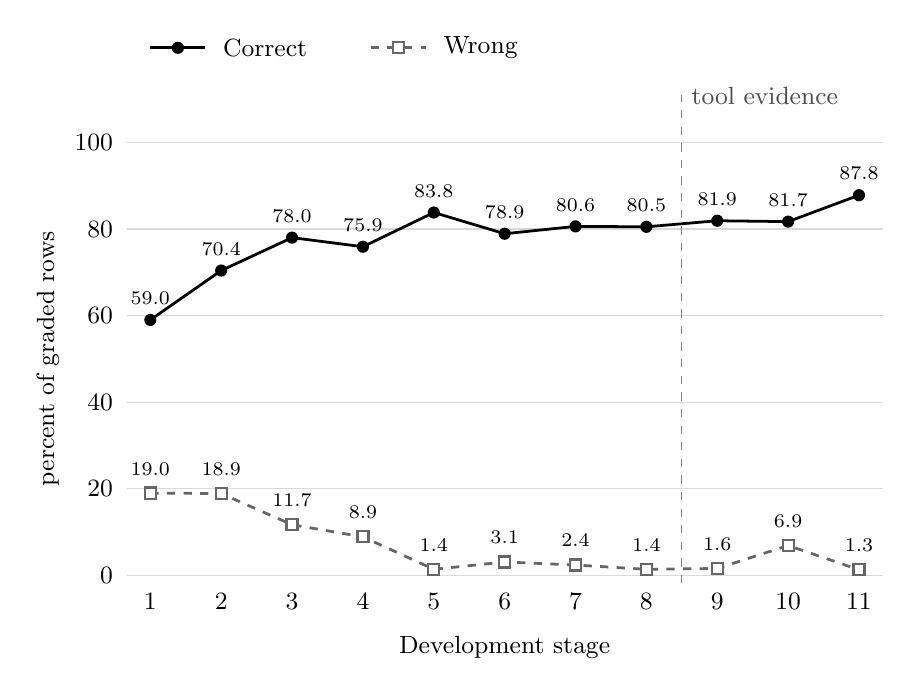
\begin{tikzpicture}[x=1cm,y=1cm,font=\small]
  \foreach \p in {0,20,40,60,80,100} {
    \draw[black!15] (-0.3,{0.055*\p}) -- (9.3,{0.055*\p});
    \node[left] at (-0.35,{0.055*\p}) {\p};
  }
  \foreach \s in {1,...,11} {
    \node[below] at ({(\s-1)*0.9},-0.1) {\s};
  }
  \node[below] at (4.5,-0.65) {Development stage};
  \node[rotate=90] at (-1.3,2.75) {percent of graded rows};
  % judges see tool output from stage 9 on
  \draw[black!50,dashed] (6.75,-0.1) -- (6.75,6.1);
  \node[anchor=south west,black!70] at (6.75,5.85) {tool evidence};
  % correct
  \draw[line width=1pt]
    (0,{0.055*59.0}) -- (0.9,{0.055*70.4}) -- (1.8,{0.055*78.0}) -- (2.7,{0.055*75.9})
    -- (3.6,{0.055*83.8}) -- (4.5,{0.055*78.9}) -- (5.4,{0.055*80.6}) -- (6.3,{0.055*80.5})
    -- (7.2,{0.055*81.9}) -- (8.1,{0.055*81.7}) -- (9.0,{0.055*87.8});
  \foreach \s/\c in {1/59.0,2/70.4,3/78.0,4/75.9,5/83.8,6/78.9,7/80.6,8/80.5,9/81.9,10/81.7,11/87.8} {
    \fill ({(\s-1)*0.9},{0.055*\c}) circle (2.2pt);
    \node[above=2pt] at ({(\s-1)*0.9},{0.055*\c}) {\scriptsize\c};
  }
  % wrong
  \draw[black!60,dashed,line width=1pt]
    (0,{0.055*19.0}) -- (0.9,{0.055*18.9}) -- (1.8,{0.055*11.7}) -- (2.7,{0.055*8.9})
    -- (3.6,{0.055*1.4}) -- (4.5,{0.055*3.1}) -- (5.4,{0.055*2.4}) -- (6.3,{0.055*1.4})
    -- (7.2,{0.055*1.6}) -- (8.1,{0.055*6.9}) -- (9.0,{0.055*1.3});
  \foreach \s/\w in {1/19.0,2/18.9,3/11.7,4/8.9,5/1.4,6/3.1,7/2.4,8/1.4,9/1.6,10/6.9,11/1.3} {
    \fill[white,draw=black!60,line width=.8pt] ({(\s-1)*0.9-0.07},{0.055*\w-0.07}) rectangle ++(0.14,0.14);
    \node[above=3pt] at ({(\s-1)*0.9},{0.055*\w}) {\scriptsize\w};
  }
  % legend
  \draw[line width=1pt] (0,6.7) -- (0.7,6.7);
  \fill (0.35,6.7) circle (2.2pt);
  \node[right] at (0.8,6.7) {Correct};
  \draw[black!60,dashed,line width=1pt] (2.8,6.7) -- (3.5,6.7);
  \fill[white,draw=black!60,line width=.8pt] (3.08,6.63) rectangle ++(0.14,0.14);
  \node[right] at (3.6,6.7) {Wrong};
\end{tikzpicture}
\caption[Correct and wrong percentages of graded rows at the eleven development stages on the 334 tuned emails]{Correct and wrong percentages of graded rows at the eleven development stages on the 334 tuned emails. The dashed vertical line marks the first stage whose grading included tool output. Grading rules and evidence changed along the way, so the stages are comparable only in direction, and none of the stages is a clean measurement. The full table, with the \textsc{Gap} shares and the state of the system at each stage, is Table~\ref{tab:live-history}.}
\label{fig:live-stages}
\end{figure}


Figure~\ref{fig:live-stages} plots the full-set results of the development period on the tuned emails (the state of the system at each stage is in Table~\ref{tab:live-history}, Appendix~\ref{app:live-history}). The rubric and the evidence available to judges changed along the way, so stages can only be compared by whether the rate went up or down. Early improvement came mostly from turning gaps into answers through newly confirmed facts (\textsc{Gap} fell from 22.1 to 10.7 percent between Stages 1 and 2). The 18.9 percent wrong rate at Stage 2 was traced to two retrieval faults (Section~\ref{sec:live-ab}). Repairing them, together with further FAQ edits, reduced \textsc{Wrong} to 11.7 percent at Stage 3. The rise at Stage 10 was partly a grading mistake. Nine of the 22 wrong rows had no invented detail, and after correcting them the wrong rate was 4.1 percent, against 1.6 percent at Stage 9. The Stage 11 figure of 87.8 percent is on the set that supplied the fixes.

The 109 real first questions and the 38 recent questions served as monitoring sets (Table~\ref{tab:live-traffic}, Appendix~\ref{app:live-traffic}). The first measurement compared the answers students had received with the build current at that time. The received answers were 40.0 percent correct and 27.0 percent wrong, against 57.7 and 4.1 percent for the build. From the first run with tool evidence on, both sets stay between about 82 and 90 percent correct, with mostly zero to three percent wrong. These questions guided fixes, so they say little about new emails.

\subsection{A/B comparisons on the live system}
\label{sec:live-ab}

Individual changes were compared in A/B runs on test containers with the same questions, two configurations and blind grading. Some comparisons use hard sets, which are emails that earlier runs answered wrongly. Figure~\ref{fig:live-ab} shows the correct rate before and after each change that reports one. The full list is Table~\ref{tab:live-ab} in Appendix~\ref{app:live-ab}.

% Correct rate before (open circle) and after (filled circle) each A/B comparison that reports one.
% x = percent * 0.085 cm; the label column is 5.2 cm wide.
\begin{figure}[htbp]
\centering
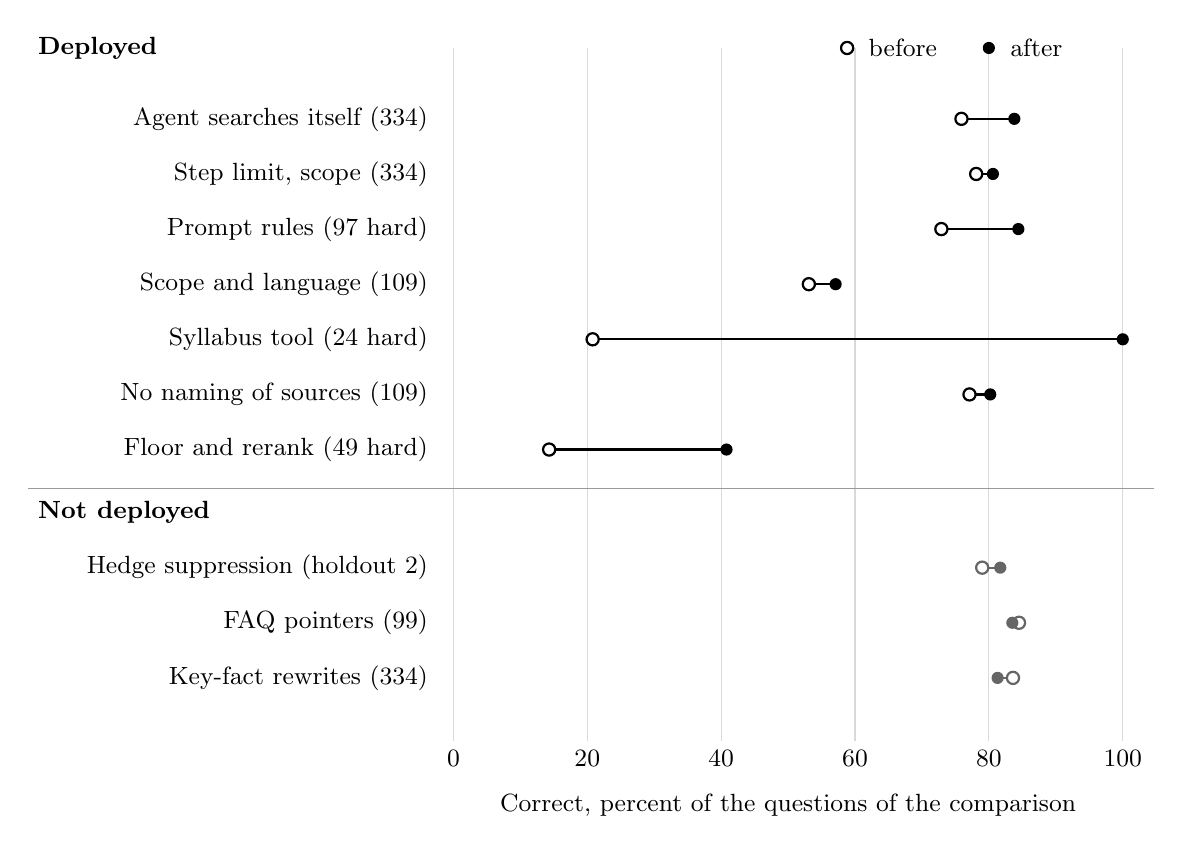
\begin{tikzpicture}[x=1cm,y=1cm,font=\small]
  \foreach \p in {0,20,40,60,80,100} {
    \draw[black!15] ({0.085*\p},0.5) -- ({0.085*\p},-8.3);
    \node[below] at ({0.085*\p},-8.3) {\p};
  }
  \node[below] at (4.25,-8.85) {Correct, percent of the questions of the comparison};
  \node[anchor=west] at (-5.4,0.5) {\textbf{Deployed}};
  \foreach \y/\lab/\b/\a in {
      -0.4/{Agent searches itself (334)}/75.9/83.8,
      -1.1/{Step limit, scope (334)}/78.1/80.6,
      -1.8/{Prompt rules (97 hard)}/72.9/84.4,
      -2.5/{Scope and language (109)}/53.1/57.1,
      -3.2/{Syllabus tool (24 hard)}/20.8/100,
      -3.9/{No naming of sources (109)}/77.1/80.2,
      -4.6/{Floor and rerank (49 hard)}/14.3/40.8} {
    \node[left,align=right] at (-0.2,\y) {\lab};
    \draw[black,line width=.8pt] ({0.085*\b},\y) -- ({0.085*\a},\y);
    \fill[white,draw=black,line width=.8pt] ({0.085*\b},\y) circle (2.2pt);
    \fill[black] ({0.085*\a},\y) circle (2.2pt);
  }
  \draw[black!40] (-5.4,-5.1) -- (8.9,-5.1);
  \node[anchor=west] at (-5.4,-5.4) {\textbf{Not deployed}};
  \foreach \y/\lab/\b/\a in {
      -6.1/{Hedge suppression (holdout 2)}/79.0/81.7,
      -6.8/{FAQ pointers (99)}/84.5/83.5,
      -7.5/{Key-fact rewrites (334)}/83.6/81.3} {
    \node[left,align=right] at (-0.2,\y) {\lab};
    \draw[black!60,line width=.8pt] ({0.085*\b},\y) -- ({0.085*\a},\y);
    \fill[white,draw=black!60,line width=.8pt] ({0.085*\b},\y) circle (2.2pt);
    \fill[black!60] ({0.085*\a},\y) circle (2.2pt);
  }
  % legend
  \fill[white,draw=black,line width=.8pt] (5.0,0.5) circle (2.2pt);
  \node[right] at (5.15,0.5) {before};
  \fill[black] (6.8,0.5) circle (2.2pt);
  \node[right] at (6.95,0.5) {after};
\end{tikzpicture}
\caption[Correct rate before and after each change of the live system, for the comparisons that report one (set size in brackets)]{Correct rate before and after each change of the live system, for the comparisons that report one (set size in brackets). Table~\ref{tab:live-ab} explains each change in one line. Open circles show the baseline and filled circles the changed configuration. ``Hard'' sets contain emails that earlier runs answered wrongly, so their baseline is low and their gains are inflated. The first row is derived from counts (7 and 20 of 49). Rejected or not deployed changes are in grey. Comparisons that report other measures (refusals, empty lookups, broken links, hedge phrases) appear only in the table in Appendix~\ref{app:live}.}
\label{fig:live-ab}
\end{figure}


Changes to evidence selection, tools and prompts each helped on some sets. The changes were measured on different sets. The floor, agent-search and second-round prompt comparisons (rules for query planning, explaining procedures and treating both meanings of a term) used hard sets, so their gains are inflated and cannot be ranked against each other. The author found the two causes of the Stage 2 wrong rate by reading the wrong answers together with the sources the bot had retrieved. One was the reranker context floor of 0.10 (passages scoring below it are dropped), which all four policies of the controlled experiment kept for FAQs. The other was reranking against the model's rewrite instead of the student's wording. In that run 106 of 334 answers had no visible sources, and these were wrong in 38 percent of graded cases (30 of 80) against 12 percent for the others (25 of 211). Lowering the floor to 0.03 and reranking against the original question gave large gains on the hard set (Table~\ref{tab:live-ab}). The reranker gives long, multi-topic emails low absolute scores even when its ranking is right. In 30 of the 49 wrongly answered emails the expected FAQ was among the candidates, but 29 of these 30 scored below 0.10. The value 0.03 was chosen by comparing three floors on the same 49 emails. The expected FAQ reached the top ten in 28.6 percent of them at 0.10, 42.9 percent at 0.03 and 44.9 percent at 0.01. The floor of 0.03 was chosen because it came close to 0.01 while still dropping the lowest-scoring passages. Only 0.10 and 0.03 were then compared end to end. These values are specific to BGE-reranker-v2-m3. Another reranker spreads its scores differently and would need its own floor. The decision model of Section~\ref{sec:live-decisions} shows this. Its scores are probabilities on a different scale, and with the same 0.03 floor it dropped loosely related passages that the cross-encoder kept. The controlled finding that selection changes do not help therefore applies only to the document threshold. Moving retrieval into the agent replaced the fixed pipeline and, on the hard set, removed most wrong answers.

Two negative results show the limits of prompt-level fixes. The hedge-suppression rule roughly halved hedge phrases, but the correct rate moved within noise and seven rows contained unsupported dates, fees or procedures. A likely explanation, which was not tested, is that the rule also suppressed legitimate uncertainty. A prompt rule against corrupting URLs did not reduce broken links, but returning short links from the tool removed them (all 19 distinct short links in the answers resolved correctly). Where a failure came from a data format, a data fix worked and an instruction did not.

\subsection{Error analysis on the final held-out set}
\label{sec:live-failures}

% Failure taxonomy of holdout 3: Gap clusters, Gap rows by evidence in context, and partial-answer causes.
% Bars: 0.2 cm per row. Label column 5.6 cm wide.
\begin{figure}[htbp]
\centering
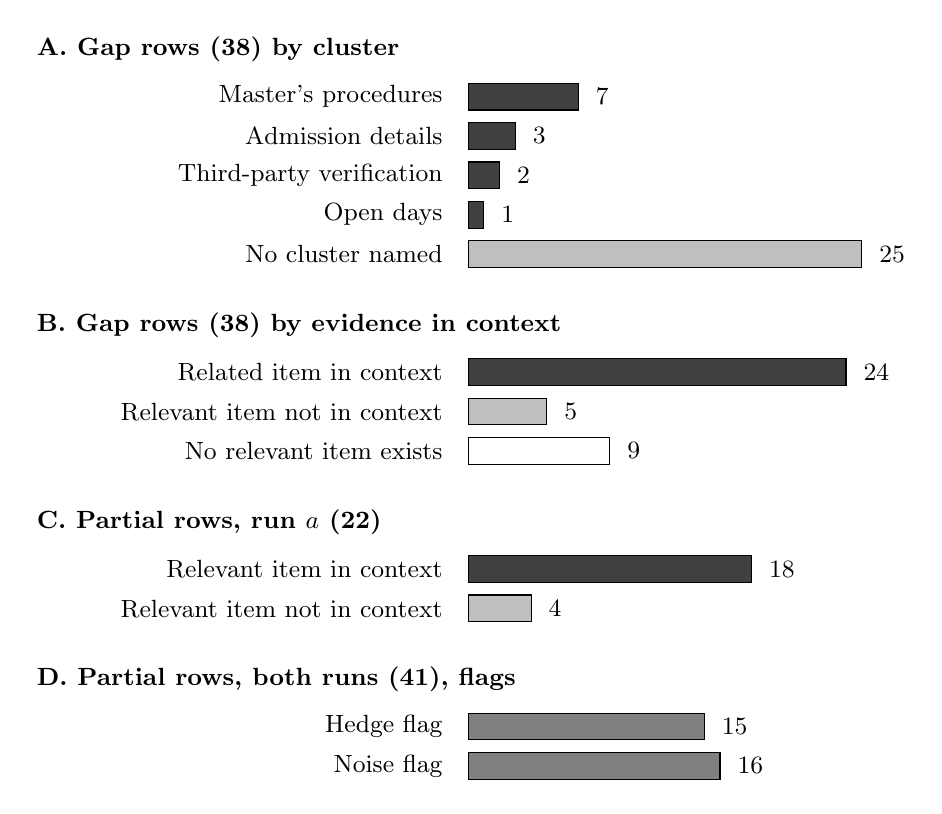
\begin{tikzpicture}[x=1cm,y=1cm,font=\small]
  % panel A
  \node[anchor=west] at (-5.6,0) {\textbf{A. \textsc{Gap} rows (38) by cluster}};
  \foreach \y/\lab/\n/\sty in {
      -0.6/{Master's procedures}/7/black!75,
      -1.1/{Admission details}/3/black!75,
      -1.6/{Third-party verification}/2/black!75,
      -2.1/{Open days}/1/black!75,
      -2.6/{No cluster named}/25/black!25} {
    \node[left] at (-0.2,\y) {\lab};
    \fill[\sty,draw=black] (0,\y-0.17) rectangle ({0.2*\n},\y+0.17);
    \node[right] at ({0.2*\n+0.1},\y) {\n};
  }
  % panel B
  \node[anchor=west] at (-5.6,-3.5) {\textbf{B. \textsc{Gap} rows (38) by evidence in context}};
  \foreach \y/\lab/\n/\sty in {
      -4.1/{Related item in context}/24/black!75,
      -4.6/{Relevant item not in context}/5/black!25,
      -5.1/{No relevant item exists}/9/white} {
    \node[left] at (-0.2,\y) {\lab};
    \fill[\sty,draw=black] (0,\y-0.17) rectangle ({0.2*\n},\y+0.17);
    \node[right] at ({0.2*\n+0.1},\y) {\n};
  }
  % panel C
  \node[anchor=west] at (-5.6,-6.0) {\textbf{C. \textsc{Partial} rows, run $a$ (22)}};
  \foreach \y/\lab/\n/\sty in {
      -6.6/{Relevant item in context}/18/black!75,
      -7.1/{Relevant item not in context}/4/black!25} {
    \node[left] at (-0.2,\y) {\lab};
    \fill[\sty,draw=black] (0,\y-0.17) rectangle ({0.2*\n},\y+0.17);
    \node[right] at ({0.2*\n+0.1},\y) {\n};
  }
  % panel D
  \node[anchor=west] at (-5.6,-8.0) {\textbf{D. \textsc{Partial} rows, both runs (41), flags}};
  \foreach \y/\lab/\n/\sty in {
      -8.6/{Hedge flag}/15/black!50,
      -9.1/{Noise flag}/16/black!50} {
    \node[left] at (-0.2,\y) {\lab};
    \fill[\sty,draw=black] (0,\y-0.17) rectangle ({0.2*\n},\y+0.17);
    \node[right] at ({0.2*\n+0.1},\y) {\n};
  }
\end{tikzpicture}
\caption[Where answers were lost on holdout 3, as row counts]{Where answers were lost on holdout 3, as row counts. Panel A: the \textsc{Gap} rows (38 in each run) that belong to the four clusters that added data could fill. The other 25 rows are not assigned to a cluster. Panel B: the same \textsc{Gap} rows of run $a$ by whether a relevant item was in the agent's context. The relevant items are mostly related passages that lack the specific fact. Panel C: the \textsc{Partial} rows of run $a$ by evidence in context. Panel D: the hedge flags (vague wording that avoids stating a rule) and noise flags (unneeded or off-topic detail) among the 41 partial answers of the two runs combined, with each flag counted separately. Relevance comes from AI judges (Section~\ref{sec:live-recall}).}
\label{fig:failure-taxonomy}
\end{figure}


On holdout 3 the largest loss is \textsc{Gap} (38 rows, 12.8 percent of all 298 rows and 14 percent of graded rows) in both runs. Next come \textsc{Partial} answers (22 and 19 rows, 41 across both runs, of which 15 were flagged for hedging and 16 for added noise, meaning unneeded or off-topic detail) and \textsc{Wrong} answers (3 and 8 rows). Figure~\ref{fig:failure-taxonomy} sorts the losses. The \textsc{Gap} rows cluster in master's procedures, third-party verification of degrees, admission details and open days. These four clusters hold 13 of the 38 rows, and added data could fill them. In run $a$, 9 of the 38 rows had no relevant item at all, 24 had a related item in context that lacked the specific fact, and 5 had a relevant item outside the context.

Partial answers have two main causes. In one, the right FAQ was retrieved but the model hedged instead of stating the rule. In the other, the model added a detail from a loosely related passage. The second holdout shows more cases, and they appeared in both identical runs. Examples include a fact buried in a large FAQ, a model that hedged although the correct FAQ was the top hit, and retrieval that missed an unusual phrasing. In other rows the model misread a context, for example by applying an admission statement to the wrong applicant, and some dates came from old announcements and were unsupported. The hedge experiment suggests that a blunt prompt rule cannot remove hedging without a cost.

For the deployed agent on fresh emails, the largest single loss is \textsc{Gap}. \textsc{Gap} rows (38 per run) outnumber wrong and partial rows combined (25 and 27), and filling a gap requires a fact confirmed by the institution. Only 9 of the 38 rows in run $a$ had no related item anywhere, so missing data is not the whole explanation. This does not contradict the controlled experiment, which held the corpus fixed and found no benefit from more context.

\subsection{Retrieval methods and recall}
\label{sec:live-recall}

This subsection measures whether the knowledge that answers an email reaches the model's context. It uses the 298 emails of holdout 3 and the live knowledge base. The knowledge base has 104 FAQs and 65 documents (2,524 chunks). Two measures are used. Hit@$k$ is the share of emails with a relevant item among the top $k$ results. MRR (mean reciprocal rank) is the average of 1/rank of the first relevant item, so higher is better for both.

\textbf{Gold standard.} Relevance was judged on one pool of candidates per email. The pool held the top three results of every ranked method, every item in the production and agent contexts, and the FAQ labels from an earlier first pass, in which an AI model marked the FAQs that answer each email. This gave 4,804 judgments. Ten Sonnet judges decided whether each item contains a fact needed for the answer. Of the 298 emails, 275 have at least one relevant item, and there are 654 relevant items, 70 percent of them FAQs. The pool included 350 FAQ labels from the earlier first pass, and the judges confirmed 298 of them. Relevance includes partial relevance, and items not judged count as non-relevant, so hit@5 and hit@10 are lower bounds. All rates are shares of the 275 emails with a relevant item.

\textbf{Methods.} BM25, a classic keyword ranking that scores passages by the query words they share, and BGE-M3 dense retrieval are the base methods. Hybrid retrieval combines both rankings by reciprocal rank fusion (RRF), which merges two ranked lists by adding 1/rank from each. HyDE searches with a hypothetical answer written by a language model. The last method is an LLM rewrite of the email into a search query. Dense, hybrid, HyDE and rewrite retrieval were also run with the BGE-reranker-v2-m3 cross-encoder re-scoring the top 30 against the original email. Two more runs show the context the model receives: the production retrieval call on the raw email, and the agent's own recorded searches replayed through production retrieval. Sonnet wrote the HyDE and rewrite texts, not the deployed model, so they show what the techniques can reach.

% Heatmap table of retrieval hit rates on holdout 3 (item level, percent of the 275 questions with a relevant item).
\begin{figure}[htbp]
\centering
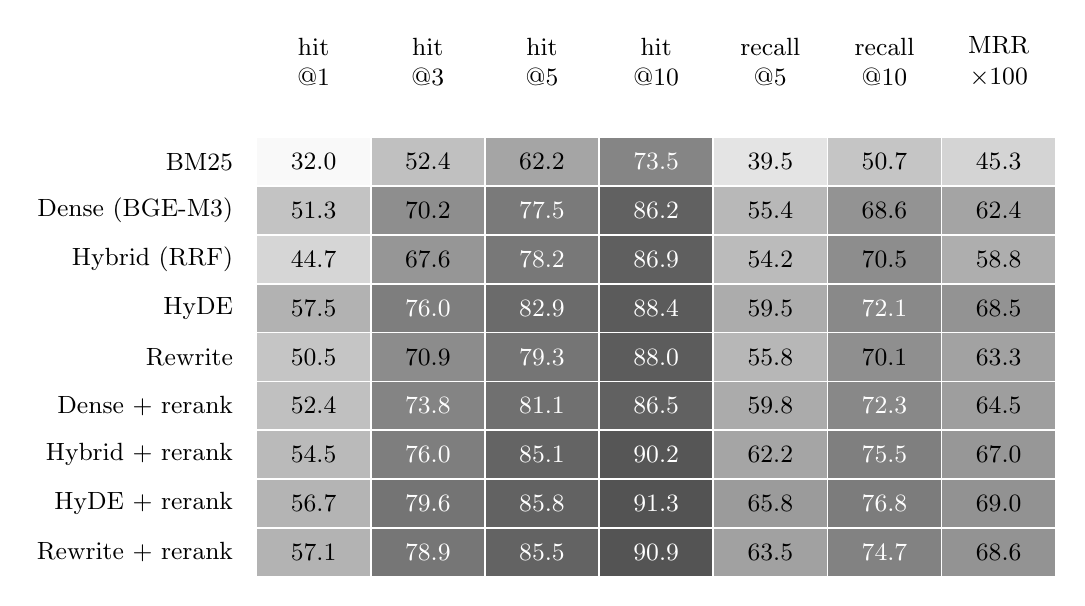
\begin{tikzpicture}[x=1cm,y=1cm,font=\small]
  \def\cw{1.45}
  \def\ch{0.62}
  \def\hc#1#2#3{%
    \pgfmathsetmacro{\sh}{max(0,(#3-30))*1.1}%
    \pgfmathparse{#3>=72?1:0}%
    \ifnum\pgfmathresult=1 \def\tc{white}\else\def\tc{black}\fi
    \node[fill=black!\sh,text=\tc,minimum width=\cw cm,minimum height=\ch cm,inner sep=0pt,draw=white,line width=.6pt] at ({3.2+#1*\cw},{-#2*\ch}) {#3};%
  }
  \foreach \c/\lab in {0/{hit\\@1},1/{hit\\@3},2/{hit\\@5},3/{hit\\@10},4/{recall\\@5},5/{recall\\@10},6/{MRR\\$\times$100}} {
    \node[align=center] at ({3.2+\c*\cw},0.65) {\lab};
  }
  \foreach \r/\name/\a/\b/\c/\d/\f/\g/\e in {
    1/{BM25}/32.0/52.4/62.2/73.5/39.5/50.7/45.3,
    2/{Dense (BGE-M3)}/51.3/70.2/77.5/86.2/55.4/68.6/62.4,
    3/{Hybrid (RRF)}/44.7/67.6/78.2/86.9/54.2/70.5/58.8,
    4/{HyDE}/57.5/76.0/82.9/88.4/59.5/72.1/68.5,
    5/{Rewrite}/50.5/70.9/79.3/88.0/55.8/70.1/63.3,
    6/{Dense + rerank}/52.4/73.8/81.1/86.5/59.8/72.3/64.5,
    7/{Hybrid + rerank}/54.5/76.0/85.1/90.2/62.2/75.5/67.0,
    8/{HyDE + rerank}/56.7/79.6/85.8/91.3/65.8/76.8/69.0,
    9/{Rewrite + rerank}/57.1/78.9/85.5/90.9/63.5/74.7/68.6} {
    \node[left] at (2.3,-\r*\ch) {\name};
    \hc{0}{\r}{\a}\hc{1}{\r}{\b}\hc{2}{\r}{\c}\hc{3}{\r}{\d}\hc{4}{\r}{\f}\hc{5}{\r}{\g}\hc{6}{\r}{\e}
  }
\end{tikzpicture}
\caption[Retrieval methods on holdout 3, measured at the item level (a chunk counts for its document)]{Retrieval methods on holdout 3, measured at the item level (a chunk counts for its document). The hit@$k$ cells give the percentage of the 275 emails with a relevant item for which a relevant item appears in the top $k$. The recall@$k$ cells give the percentage of an email's relevant items that appear in the top $k$, averaged over the 275 emails. The last column is the mean reciprocal rank multiplied by 100. Darker cells are higher values. The 4 bottom rows add the cross-encoder reranker on the top 30 candidates.}
\label{fig:recall-heatmap}
\end{figure}


Figure~\ref{fig:recall-heatmap} gives the ranking quality of the nine methods. BM25 is weakest. Every other method finds a relevant item in the top ten for 86 to 91 percent of the emails.

% In-context recall on holdout 3: production retrieval versus the agent's own searches.
\begin{figure}[htbp]
\centering
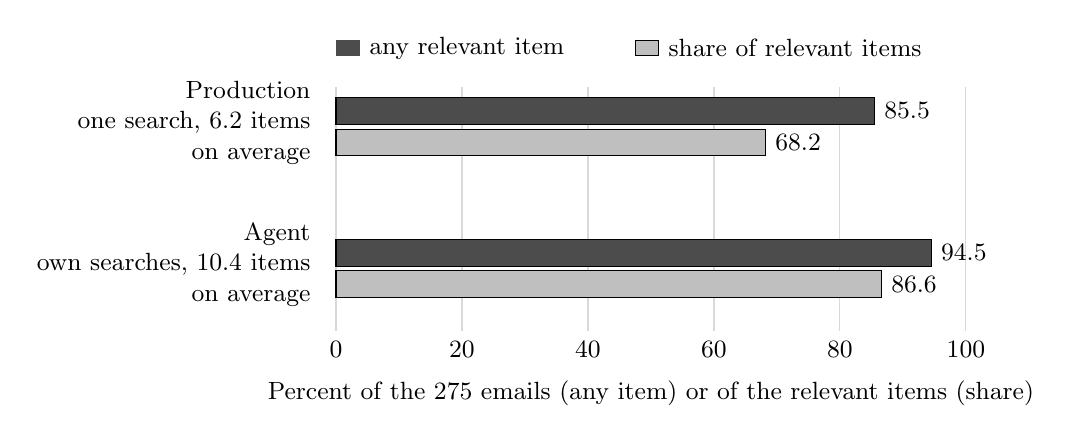
\begin{tikzpicture}[x=1cm,y=1cm,font=\small]
  \foreach \p in {0,20,40,60,80,100} {
    \draw[black!15] ({\p*0.08},0.6) -- ({\p*0.08},-2.5);
    \node[below] at ({\p*0.08},-2.5) {\p};
  }
  \node[below] at (4,-3.0) {Percent of the 275 emails (any item) or of the relevant items (share)};
  \node[left,align=right] at (-0.2,0.15) {Production\\one search, 6.2 items\\on average};
  \node[left,align=right] at (-0.2,-1.65) {Agent\\own searches, 10.4 items\\on average};
  \foreach \y/\v/\f in {0.3/85.5/black!70, -0.1/68.2/black!25, -1.5/94.5/black!70, -1.9/86.6/black!25} {
    \fill[\f,draw=black] (0,\y-0.17) rectangle ({\v*0.08},\y+0.17);
    \node[right] at ({\v*0.08},\y) {\v};
  }
  \fill[black!70] (0,1.0) rectangle (0.3,1.2);
  \node[right] at (0.3,1.1) {any relevant item};
  \fill[black!25,draw=black] (3.8,1.0) rectangle (4.1,1.2);
  \node[right] at (4.1,1.1) {share of relevant items};
\end{tikzpicture}
\caption[Relevant knowledge in the model's context on holdout 3]{Relevant knowledge in the model's context on holdout 3. Production retrieval makes one call on the raw email, and the agent searches about 1.7 times per answer. The dark bars give the percentage of emails with at least one relevant item in context, the light bars the share of all relevant items that reached the context.}
\label{fig:recall-context}
\end{figure}


Figure~\ref{fig:recall-context} shows what reaches the model. One production search on the raw email puts a relevant item in context for 85.5 percent of the emails and covers 68.2 percent of all relevant items, with 6.2 items on average. The agent searches about 1.7 times per answer and brings 10.4 items on average. It reaches 94.5 and 86.6 percent.

% Grades of holdout 3 (run a) split by whether a relevant item reached the agent's context.
\begin{figure}[htbp]
\centering
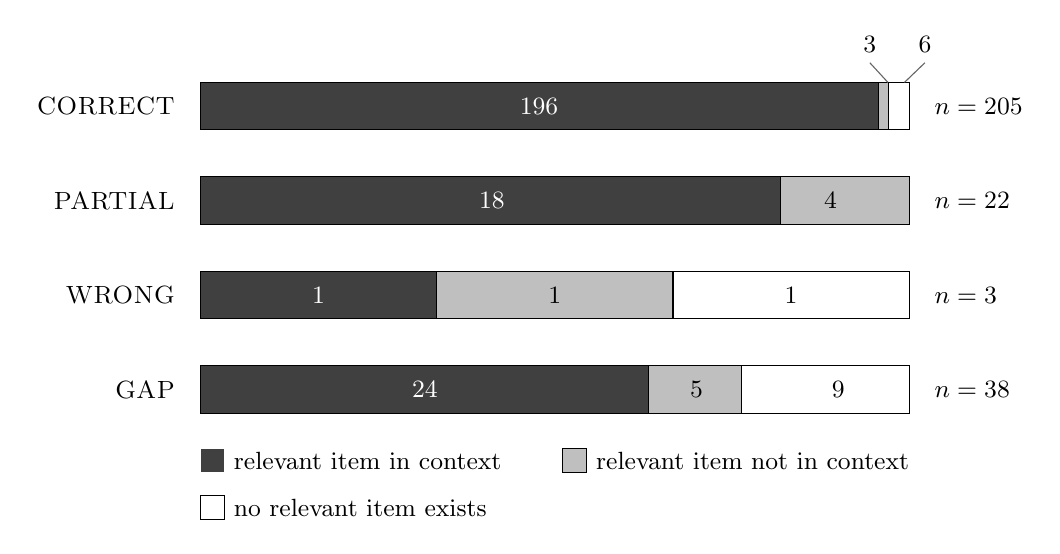
\begin{tikzpicture}[x=1cm,y=1cm,font=\small]
  \def\w{0.09}
  \fill[black!75] (0,-4.65) rectangle (0.3,-4.35);
  \node[right] at (0.3,-4.5) {relevant item in context};
  \fill[black!25,draw=black] (4.6,-4.65) rectangle (4.9,-4.35);
  \node[right] at (4.9,-4.5) {relevant item not in context};
  \fill[white,draw=black] (0,-5.25) rectangle (0.3,-4.95);
  \node[right] at (0.3,-5.1) {no relevant item exists};
  \foreach \y/\g/\a/\b/\c in {0/CORRECT/196/3/6, -1.2/PARTIAL/18/4/0, -2.4/WRONG/1/1/1, -3.6/GAP/24/5/9} {
    \pgfmathtruncatemacro{\n}{\a+\b+\c}
    \pgfmathsetmacro{\xa}{\a/\n*9}
    \pgfmathsetmacro{\xb}{(\a+\b)/\n*9}
    \node[left] at (-0.2,\y) {\textsc{\g}};
    \node[right] at ({100*\w+0.2},\y) {$n=\n$};
    \fill[black!75] (0,\y-0.3) rectangle (\xa,\y+0.3);
    \ifnum\b>0 \fill[black!25] (\xa,\y-0.3) rectangle (\xb,\y+0.3);\fi
    \ifnum\c>0 \fill[white] (\xb,\y-0.3) rectangle ({100*\w},\y+0.3);\fi
    \draw (0,\y-0.3) rectangle ({100*\w},\y+0.3);
    \ifnum\b>0 \draw (\xa,\y-0.3) -- (\xa,\y+0.3);\fi
    \ifnum\c>0 \draw (\xb,\y-0.3) -- (\xb,\y+0.3);\fi
  }
  % counts on the wide segments
  \node[text=white] at (4.3,0) {196};
  \node[text=white] at (3.7,-1.2) {18};
  \node at (8.0,-1.2) {4};
  \node[text=white] at (1.5,-2.4) {1};
  \node at (4.5,-2.4) {1};
  \node at (7.5,-2.4) {1};
  \node[text=white] at (2.85,-3.6) {24};
  \node at (6.3,-3.6) {5};
  \node at (8.1,-3.6) {9};
  % counts on the narrow segments of CORRECT
  \draw[black!60] (8.73,0.3) -- (8.5,0.55);
  \node[above] at (8.5,0.55) {3};
  \draw[black!60] (8.94,0.3) -- (9.2,0.55);
  \node[above] at (9.2,0.55) {6};
\end{tikzpicture}
\caption[Grades of holdout 3 (run $a$) by whether a relevant item reached the agent's context]{Grades of holdout 3 (run $a$) by whether a relevant item reached the agent's context. Each bar is scaled to 100 percent of the graded rows of its grade, and the numbers are row counts. \textsc{N/A} rows are omitted. Most answers that were not fully correct had a relevant item in context.}
\label{fig:error-attribution}
\end{figure}


Figure~\ref{fig:error-attribution} joins these results with the grades of run $a$: a relevant item was in context for 196 of 205 \textsc{Correct} answers and for 18 of 22 \textsc{Partial} answers.

\textbf{Findings.} Both the reranker and HyDE raise the top ranks, and HyDE with the reranker is best (hit@10 91.3 percent, MRR 0.69). Retrieval misses explain at most about 4 percent of the holdout-3 answers (13 of 298 rows). These are the rows of run $a$ with a relevant item outside the context: 3 \textsc{Correct}, 4 \textsc{Partial}, 1 \textsc{Wrong} and 5 \textsc{Gap}. Partial answers are mostly answer-construction failures (18 of 22 had a relevant item in context), in line with the controlled finding. \textsc{Gap} is mostly missing knowledge, although 24 of the 38 \textsc{Gap} rows had an item judged relevant in context. The judges were less strict and also marked passages that were only about the same topic.

\subsection{Reranking with a decision model}
\label{sec:live-decisions}

This subsection tests a hosted decision model (the OpenAI Decisions API with GPT-6 Luna) in place of the production cross-encoder. For each candidate passage the model answers one yes-or-no question: does the passage contain information needed to answer? The returned probability is the ranking score. Table~\ref{tab:live-decisions} gives two tests. The first orders the dense top 20 candidates of the 275 holdout-3 emails with a relevant item and scores the order against the combined AI labels. The second runs the full agent twice on 100 random holdout-3 emails (fixed seed). One run uses the cross-encoder. In the other, every rerank call is replaced by the decision model, with the floor of 0.03 and the limit of ten results unchanged. Four Sonnet judges graded both arms blind and side by side.

\begin{table}[htbp]
\centering
\caption[Cross-encoder against decision-model reranking]{Cross-encoder against decision-model reranking. Ranking: item-level scores against the combined AI relevance labels, 275 emails, dense top 20 candidates. Answers: full agent on 100 holdout-3 emails, graded by Sonnet. $C$, $P$, $W$ are \textsc{Correct}, \textsc{Partial} and \textsc{Wrong} counts, and percentages are of graded rows. Context is per search.}
\label{tab:live-decisions}
\small
\begin{tabular}{@{}lrrr@{}}
\toprule
 & Dense order & Cross-encoder & Decision model \\
\midrule
\multicolumn{4}{@{}l}{\textit{Ranking quality (275 emails)}} \\
hit@1 (\%) & 51.3 & 52.7 & 68.7 \\
hit@3 (\%) & 70.2 & 73.5 & 82.9 \\
hit@5 (\%) & 77.5 & 81.5 & 84.4 \\
MRR & 0.620 & 0.645 & 0.759 \\
\midrule
\multicolumn{4}{@{}l}{\textit{Answers (100 emails)}} \\
$C$ / $P$ / $W$ / \textsc{Gap} / N/A & n/a & 70 / 8 / 1 / 15 / 6 & 65 / 9 / 4 / 16 / 6 \\
Correct (\%) & n/a & 74.5 & 69.1 \\
Wrong (\%) & n/a & 1.1 & 4.3 \\
Sources per search & n/a & 6.9 & 5.2 \\
Characters per search & n/a & 17,174 & 10,096 \\
\bottomrule
\end{tabular}
\end{table}

The decision model ranks much better against the AI labels. At hit@1, 63 emails favor it and 19 favor the cross-encoder (sign test $p\approx10^{-6}$). With the top 20 hybrid candidates its hit@1 rose to 77.1 percent against 54.5 for the cross-encoder. The cross-encoder hit@1 of 52.7 here reranks 20 candidates, so it differs from the 52.4 of dense plus rerank in Figure~\ref{fig:recall-heatmap}, which reranks the top 30. A four-level score instead of a yes-or-no question gave 72.0. A ranking request for 20 passages took a median of 0.3 seconds, and the 275 requests cost about 0.20 US dollars.

The better ranking did not produce better answers. The cross-encoder arm was better on 12 rows and worse on 6, so 74.5 against 69.1 percent correct is not significant (sign test $p=0.24$), and the trend points the other way. Loosely related passages receive probabilities near zero, so the unchanged floor removes them and the context shrinks by about 40 percent in characters. The swap would need a tuned floor or a fixed number of results before it could pay off.

Three limits apply. The relevance labels come from AI judges using a rule similar to the decision model's question, which favors an LLM-based ranker. The end-to-end test has only 100 emails and called the model directly through OpenAI instead of through the gateway of the earlier live runs, so its absolute rates are not comparable with Table~\ref{tab:live-holdout}. Candidates are limited to the dense top 20.

\subsection{Multi-turn memory}
\label{sec:live-memory}

This test checks whether the agent uses earlier turns. An AI model wrote sixty short conversations of two to three user turns from the FAQ snapshot, 15 for each of four types. In ellipsis, the follow-up omits what it refers to. In profile, the student gave a fact earlier. In correction, the student corrects or narrows an earlier question, for example from undergraduate to master's fees. In reference, the follow-up points back to an earlier answer. Each conversation was asked turn by turn with the bot's own earlier answers in the request, as the web client does. The last turn was also asked alone as a control. Three Sonnet judges judged whether the answer used the earlier context and was correct against the expected facts.

\begin{table}[htbp]
\centering
\caption{Multi-turn memory test by conversation type: items, answers graded correct with history, and items whose last turn, asked alone as a control, could already be answered without history (``Control answered'').}
\label{tab:live-memory}
\small
\begin{tabular}{@{}lrrr@{}}
\toprule
Type & Items & Correct & Control answered \\
\midrule
Ellipsis & 15 & 14 & 8 \\
Profile & 15 & 15 & 4 \\
Correction & 15 & 14 & 1 \\
Reference & 15 & 15 & 5 \\
\midrule
All & 60 & 58 & 18 \\
\bottomrule
\end{tabular}
\end{table}

As Table~\ref{tab:live-memory} shows, the agent used the earlier context in all 60 conversations and answered 58 correctly. The other two were \textsc{Partial}. In 18 of the 60 items the last turn could be answered alone, so these items do not test memory and act as controls. The other 42 need the earlier turns and are the real memory test. Context was used in 42 of 42 and the answer was correct in 41 of 42. The test covers memory within one conversation only.

\subsection{Limitations of the live evaluation}
\label{sec:live-limits}

\begin{itemize}
  \item \textbf{AI judges only.} No human labels exist. Identical runs on holdout 2 differ on 12 percent of rows, and judges were wrong on invented details.
  \item \textbf{Judge model and rubric.} All five clean runs are Sonnet-graded under the current rubric, but Opus and Sonnet agree on only 81.6 percent of rows, so absolute rates depend on the judge by a few points. The Opus figures for holdout 1 (older rubric), the tuned set and the second measurement of holdout 2 are not comparable with the clean rows.
  \item \textbf{Partial automatic check.} The script checks only dates, amounts, URLs and email addresses. It skipped the second measurement of holdout 2 and the hedge experiment.
  \item \textbf{Contamination.} Only holdout 3 and the first measurements on holdouts 1 and 2 are clean. The tuned emails overstate quality by about 11 points, and the monitoring sets guided fixes.
  \item \textbf{Population.} Archive emails are written to staff rather than a chatbot, and the traffic set is small.
  \item \textbf{Moving targets.} The knowledge base grew from 74 to 104 FAQs, and the agent, prompts and tools changed. Runs of different stages therefore compare different systems against different references. The full live configuration, including provider-side behavior, cannot be replayed.
  \item \textbf{Retrieval and decision-model tests.} Relevance labels are combined AI judgments, the end-to-end comparison has 100 emails and a different API route, and HyDE and rewrite texts came from a different model than the deployed one.
  \item \textbf{Memory test.} The items are synthetic, short and AI-graded.
  \item \textbf{Scope and data.} Outside the memory test, conversations, user feedback and satisfaction are not measured, and the chatbot logs cannot be released.
\end{itemize}

The evidence supports only a limited statement. AI judges rated the deployed agent correct on roughly three quarters of graded fresh emails, against a knowledge base of confirmed facts that changed during development. Human judges might give different rates.

\paragraph{Summary.}
\begin{itemize}
  \item On clean held-out emails the agent was graded correct on 70.5 to 77.3 percent of graded questions and wrong on 0.8 to 3.0 percent. The tuned set overstates this by about 11 points.
  \item Evidence selection, tool and prompt changes each helped on some sets, and the gains cannot be ranked because the sets differ. Data fixes worked where instructions did not.
  \item The largest single loss is \textsc{Gap} (38 rows), which mostly means missing knowledge. Retrieval misses explain at most about 4 percent of answers.
  \item A decision-model reranker ranks better against AI labels but gave no better answers. With the cross-encoder 74.5 percent were correct, and with the decision model 69.1 percent, a difference within chance. In a synthetic test the agent used history in 42 of 42 real memory items and answered 41 correctly.
\end{itemize}
